\subsection{Hybrid Model Design for Text Prediction}\label{subsec:mt:hybrid-model-design}
To address the limitations of token-based models like GPT-2 in handling incomplete inputs and achieving real-time performance,
we implemented a hybrid system that combines a lightweight, character-level LSTM model with GPT-2.
This hybrid design leverages the strengths of both models, enabling efficient and accurate predictions for typing assistance tasks.

The LSTM model focuses on character-level predictions, which are particularly effective for completing partial words.
It takes an input sequence of characters, processes them through recurrent layers, and predicts the most likely next character at each timestep.
For example, given an input like ``ligh'', the LSTM predicts the following characters
(`t', `w', `e', `i', `g', `h', `t') iteratively until a space character or punctuation is encountered.

The prediction process involves:

\begin{enumerate}
\item Converting each character into an index in the vocabulary (English alphabet, numbers, and special characters), and embedding the indices into a dense representation.
\item Processing the embedded sequence through LSTM layers that retain context over the input.
\item Generating a probability distribution over the vocabulary for the next character at each timestep, selecting the character with the highest probability.
\end{enumerate}
This iterative mechanism allows the LSTM to generate highly accurate character-level completions, even for incomplete inputs.

In the hybrid system, inputs are first processed by the LSTM. If the LSTM produces a non-empty result (non-space or punctuation character), it is returned directly to the user.
Otherwise, the input is passed to GPT-2, which provides context-aware phrase completions or generates predictions for longer, more complex inputs.
By delegating simpler tasks to the LSTM, the system achieves lower latency and reduces computational load on GPT-2.

\subsection{Knowledge Distillation}
Knowledge Distillation is a technique for transferring knowledge from a large, complex model (teacher model) to a smaller,
more efficient model (student model).
The key idea is that the student model can achieve comparable performance to the teacher model by learning soft labels of the teacher:
probability distributions instead of learning the true labels only.
This allows the student to learn intermediate representations from the teacher.
The loss function of knowledge distillation can be expressed as:

\begin{equation}
    L_{\text{KD}} = \alpha L_{\text{CE}}(y, \hat{y}) + (1 - \alpha) T^2 L_{\text{KL}}(q_t, q_s)
    \label{eq:kd-loss}
\end{equation}

where $L_{\text{CE}}(y, \hat{y})$ represents the loss between prediction probability distribution $\hat{y}$ and true labels $y$ using traditional cross entropy loss.
$L_{\text{KL}}(q_t, q_s)$ expresses the difference between the output distributions of the student and the teacher.
$T$ is the temperature hyperparameter, used to soften softmax distributions of $q_t$ and $q_s$.
Finally, $\alpha$ controls the balance between different kinds of losses.

BART-large-CNN~\cite{lewis2019bart} was pre-trained and fine-tuned on the CNN Daily Mail dataset and has a powerful ability of text summarization.
It has 12 Transformer encoder layers and 12 Transformer decoder layers, the model being in total of 1.51GB\@.
GPT-2~\cite{radford2019language} was a pre-trained autoregressive decoder model using a causal language masking objective,
containing 12 Transformer decoder layers with a total size of 0.548 GB. We extracted the layers 0, 2, 5, 7, 9, 11
from the encoder/decoder to form the student's encoder/decoder, thereby halving the model's storage.
Weight state dicts of these layers are also loaded to avoid pre-training from scratch.

In our implementation, we chose to use \texttt{MSE} to match the logits output at each hidden layer
as described in~\cite{shleifer2020pre} since this can encourage the student to even match teacher hidden states.
The loss function is updated as follows,
where we want the student to generate hidden layers weights as comparable to the teacher as possible:

\begin{equation}
    L_{\text{KD}} = \alpha L_{\text{CE}}(y, \hat{y}) + \beta L_{\text{MSE}(hid_t, hid_s)} + \gamma T^2 L_{\text{KL}}(q_t, q_s)
    \label{eq:kdmse-loss}
\end{equation}

For the $\alpha, \beta, \gamma, T$ hyperparameters, we set $\alpha$ to 0.1, $\beta$ to 3, $\gamma$ to 0.8,
and $T$ to 2, since we aim to maximize the hidden state learning by the student from the teacher.

\begin{figure*}[hbpt]
    \centering
    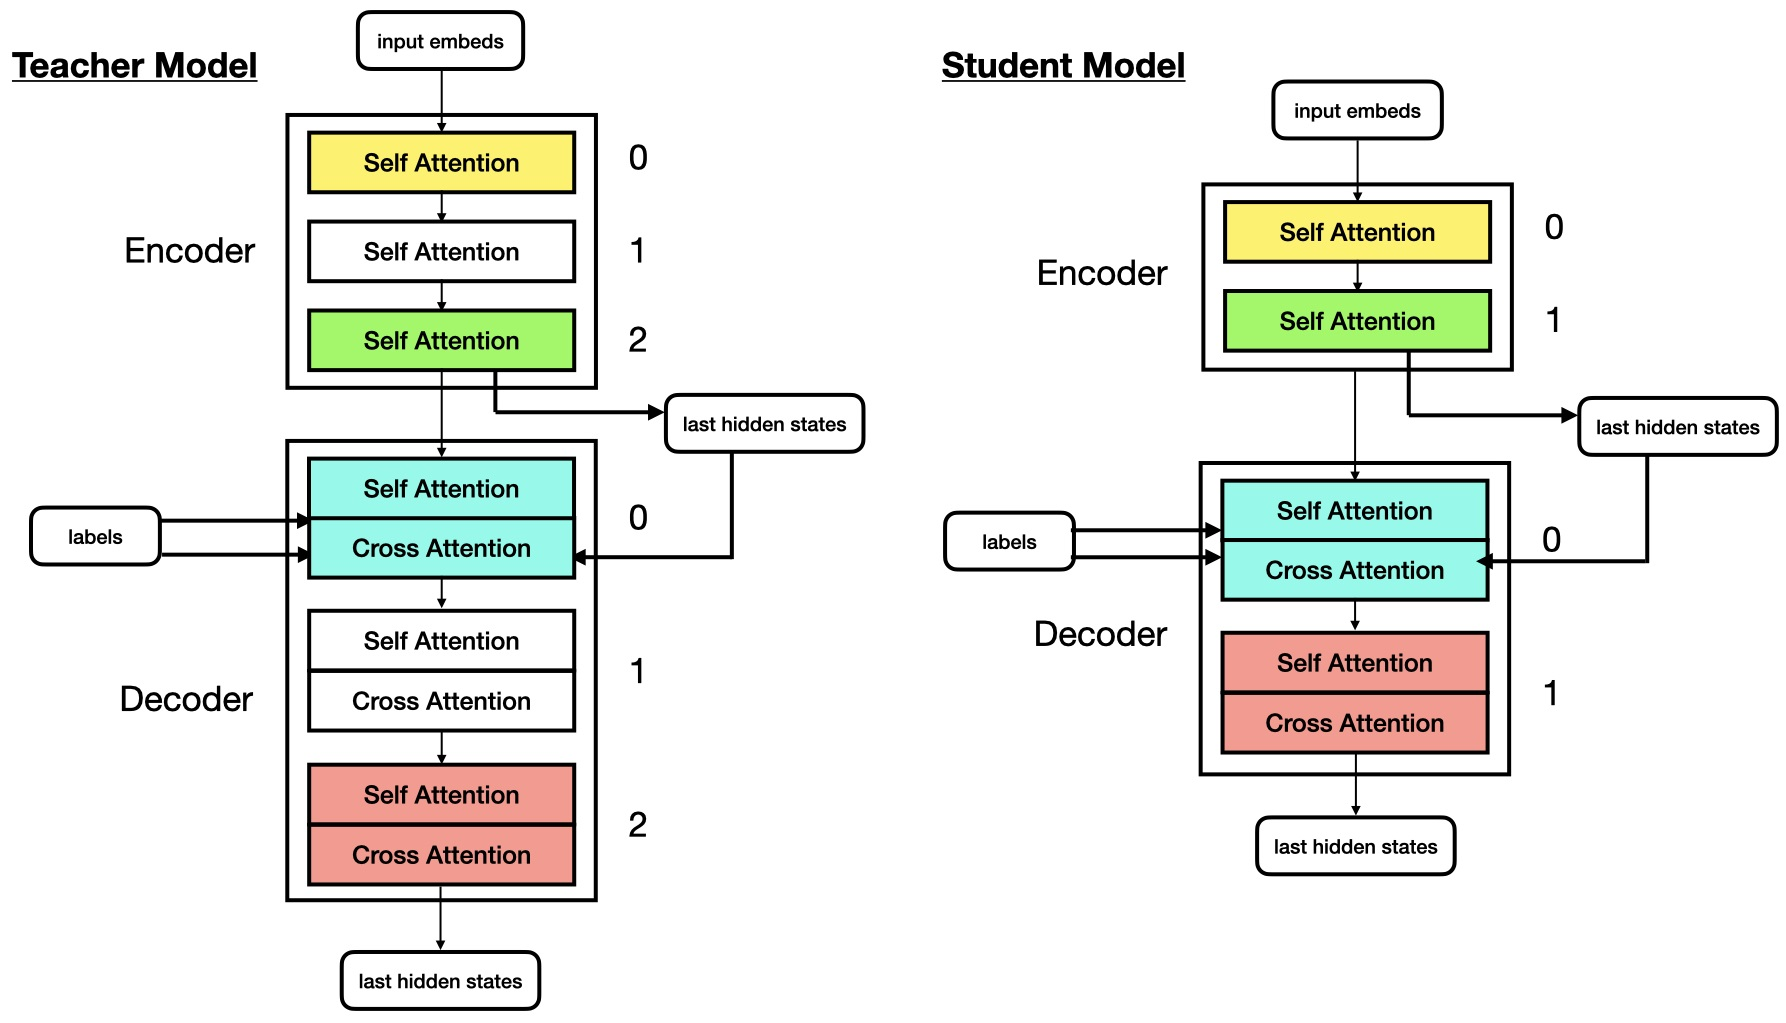
\includegraphics[width=0.9\linewidth]{images/0.001}
    \caption{Example of distillation of Encoder-Decoder model, e.g. BART-large}
    \label{fig:sub1}
\end{figure*}

\begin{figure}[hbpt]
    \centering
    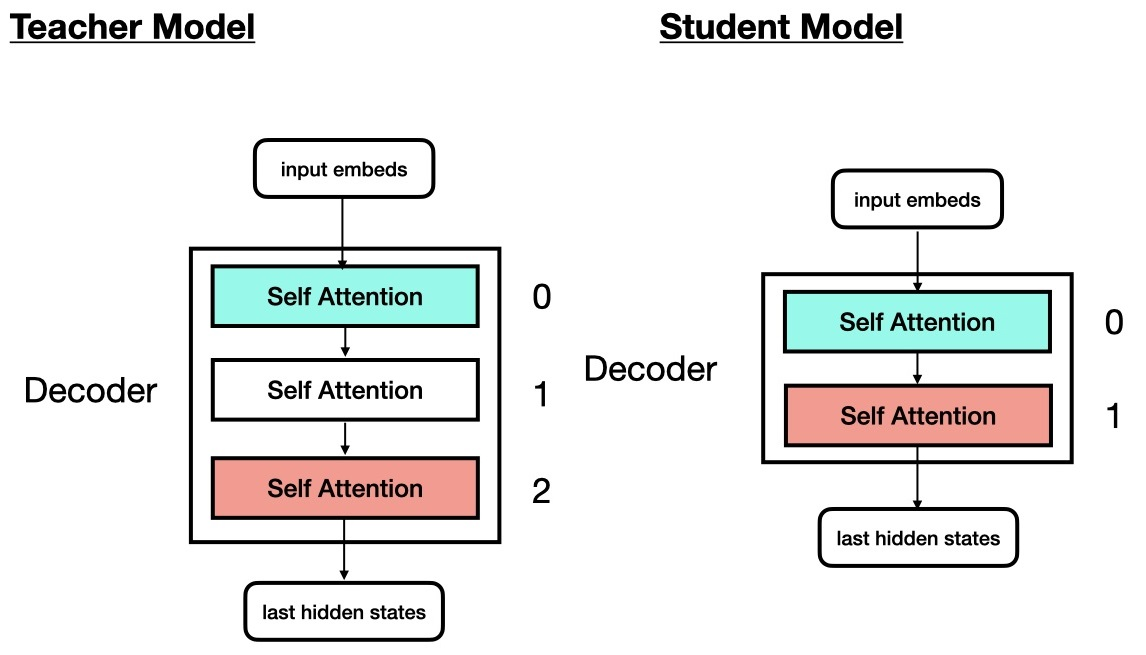
\includegraphics[width=0.9\linewidth]{images/0.002}
    \caption{Example of distillation of Decoder-Only model, e.g. GPT-2}
    \label{fig:sub2}
\end{figure}

As shown in Figure~\ref{fig:sub1}, this image illustrates an example encoder-decoder Transformer (e.g.\ BART) teacher model with 3 layers for each on the left.
On the right a distilled student model extracts the first and last layers of the teacher's encoder and decoder (using the same colors) and forms a new encoder and decoder.
Arrows in this figure show the data flow: \texttt{input embeds} are the text embedding input, which will become \texttt{Q,K,V} in encoders.
Encoder's last hidden layer states will be transformed to \texttt{K,V} used in cross-attention of decoder layers, and the \texttt{labels} are fed as \texttt{Q,K,V}
in self-attention but as \texttt{Q} only in cross-attention of decoder layers.

Figure~\ref{fig:sub2} presents an example 3-layer decoder-only Transformer (e.g.\ GPT-2) teacher model on the left,
which is much simpler than the previous one since decoder-only models can choose not to use cross-attention, meaning it only leverages self-attention.
On the right a distilled student model extracts the first and last layers of the teacher's decoder (using same colors) and forms a new decoder.
\texttt{input embeds} will become \texttt{Q,K,V} in decoders.
Finally the final logits generated by the decoder will be compared with the original text embeddings using cross entropy to calculate the loss because of autoregression.


\subsection{Movement Pruning}\label{subsec:mt:movement-pruning}
Pruning is a model optimization technique aimed at reducing the size and computational complexity of deep learning models by removing less important parameters or structures.
There are several different classification approaches for pruning, including by granularity (weight, neuron, channel, layer),
by timing (pre-training, during training, post-training), and by target (structural, unstructural).
Our pruning strategy focuses on neurons in FFN layers and attention heads in \texttt{QKV} projection layers.
Specifically, we train pruning masks for both FFN and \texttt{QKV} projections separately, and finally perform pruning using the masks.
Therefore, our approach can be categorized as structural movement pruning, taking neurons and attention heads as the minimum granularity.

We assign a uniformly drawn score to each neuron in an FFN layer and to each head in an attention layer.
Each time during forward passes, we use a threshold \texttt{K} to select the top \texttt{K}
smallest scores and drop the corresponding neurons and attention heads by transforming the scores into masks.
Regarding neurons and attention heads as pruning granularity,
we should notice that once we have determined which attention head is useless,
we should remove that same head from all \texttt{QKV} projections and the final output projection in the current attention.
Also for FFN layers that contain two linear layers \texttt{fc1} and \texttt{fc2},
once we have decided which neuron can be pruned in \texttt{fc1},
we must remove the corresponding neuron defined in \texttt{fc2}.
Therefore, we call our trained scores ``shared score'' or ``shared mask'',
since they are shared among \texttt{QKV} attention projections, and among FFN layers.

During the training process in order to find the best shared masks in the Transformer,
we will apply the current shared masks in forward and backward passes to train learnable shared masks.
However, the masking operation is not differentiable since it zeros out all corresponding attention heads
and set them to zero as inactive heads during forward passes.
To solve this, we applied STE, which stands for straight-through estimator techniques to estimate gradients
during backward passes so that the scores can be updated properly.
Therefore, the most important neuron or attention heads must have the highest score theoretically due to natural selection.
Additionally, we implemented a dynamic threshold scheduler for threshold $T$ for the movement pruning trainer, as shown in Eq.~\ref{eq:threshold}.
For instance, in our setup, we aim to prune 30\% of the attention heads in the Transformer and 60\% of the neurons in FFN layers.
To minimize abrupt performance degradation, the scheduler gradually increases the total masking threshold from 0\% to 30\%
following a cubic curve for masked attention heads.
The thresholds will reach their peek at 85\% of the training progress and stay at the peek
until the end and use the remaining 15\% of the progress for fine-tuning, as shown in Figure~\ref{fig:sub3}.

\begin{equation}
T = T_{\text{init}} + (T_{\text{final}} - T_{\text{init}}) \times (1 - \text{progress})^3
\label{eq:threshold}
\end{equation}


Figures~\ref{fig:neuron_pruning} and~\ref{fig:attention_head_pruning} show pruning results for an FFN layer and a decoder layer, respectively.
In Figure~\ref{fig:neuron_pruning}, darker colors indicate the neurons that have been pruned,
while in Figure~\ref{fig:attention_head_pruning}, darker colors highlight pruned self-attention and cross-attention heads.

\begin{figure}[hbpt]
    \centering
    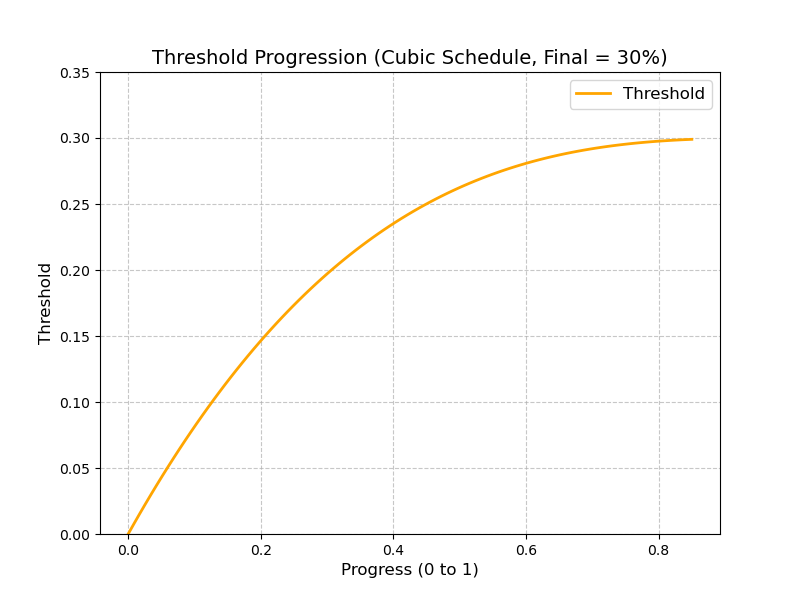
\includegraphics[width=0.9\linewidth]{images/1}
    \caption{Movement Threshold Scheduler for Attention Layers}
    \label{fig:sub3}
\end{figure}

\begin{figure}[h!]
    \centering
    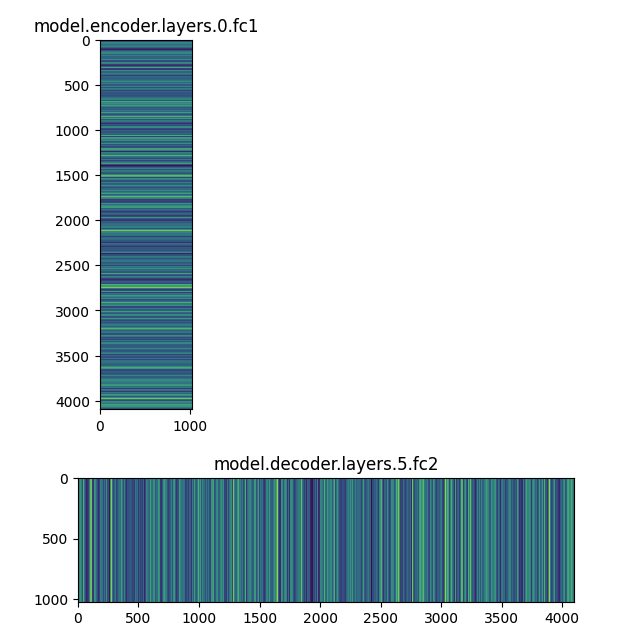
\includegraphics[width=0.9\linewidth]{images/pruning1}
    \caption{Sample Neuron Pruning for FFN}
    \label{fig:neuron_pruning}
\end{figure}

\begin{figure}[h!]
    \centering
    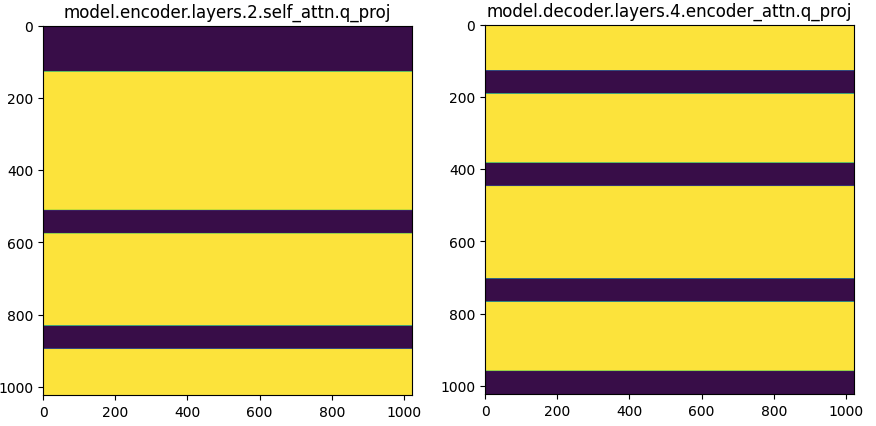
\includegraphics[width=0.9\linewidth]{images/pruning2}
    \caption{Sample Attention Head Pruning for Self-Attention and Cross-Attention in Decoder.}
    \label{fig:attention_head_pruning}
\end{figure}


\subsection{Quantization}
Quantization can reduce the precision of numbers used to present parameters or activations.
By converting high-precision floating-point numbers (FP32, FP64) to lower precision (INT8, FP16),
quantization reduces the memory footprint and computational requirements of a model,
making it more efficient for deployment on resource-constrained devices like edge or mobile devices.
Types of quantization include post-training quantization (PTQ), and quantization-aware training (QAT).
To map FP32, for instance, to INT8, we can convert floating point values into quantized space using linear mapping strategy, as expressed below:


\begin{gather}
\begin{split}
    r &= S(q-Z) \\
    q &= \operatorname{round}\left(\frac{r}{S} + Z\right)
\end{split}
\end{gather}

where $r$ and $q$ are the number before and after quantization; $S$ and $Z$ are scale and zero-point.
The linear mapping is referred to as symmetric or asymmetric mapping, depending on whether $Z$ is zero,
as shown in Figure~\ref{fig:sub4}, where a symmetric range is converted to
a symmetric INT8 range on the left and an asymmetric range is mapped to an asymmetric INT8 range.

\begin{figure}[hbpt]
    \centering
    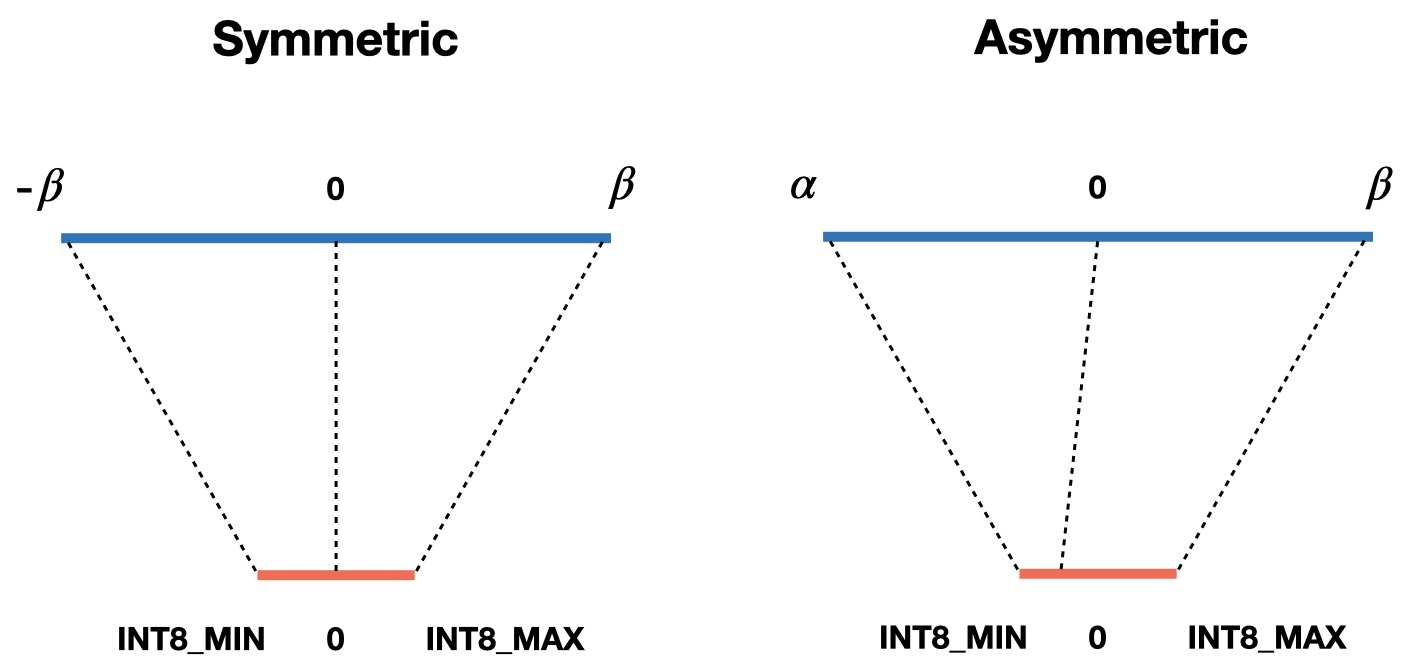
\includegraphics[width=\linewidth]{images/0.003}
    \caption{Linear Mapping with or without Zero-point}
    \label{fig:sub4}
\end{figure}

After mapping FP32 to INT8, which is PTQ, the memory footprint is significantly reduced;
however, this comes at the cost of precision and performance degradation.
To compensate for the degradation, calibration can be performed by feeding real data
into the quantized model to estimate and adjust weight ranges.

Another approach for the model to adjust for quantization errors is to use online quantization techniques,
for instance, QAT, instead of the offline PTQ method.
QAT involves training the model with quantization simulated during the process to improve performance after quantization.
Despite weights being quantized to INT8, during the forward process weights are still represented as FP32 to adjust for quantization errors.
After QAT, the model learns to compensate for quantization errors, ensuring minimal performance degradation,
followed by PTQ after training to convert the model to an INT8 format, and inference is performed using INT8 precision.

Our approach follows the above description, performing QAT first, followed by PTQ.
To implement QAT, We designed a \texttt{QLinear} layer to substitute the original \texttt{torch.nn.Linear} layers
to perform quantization-aware training.
There was a similar problem as described in Subsection~\ref{subsec:mt:movement-pruning}:
the linear mapping process, as we call it \texttt{affine}, leveraging \texttt{round} and \texttt{clamp} operations,
is non-differentiable.
We applied the same approach described above: STE to estimate the backward gradient for our \texttt{QLinear} layers
to learn and gradually adjust for quantization errors.
We rewrote the backward function for the $XW + b$ linear operation, plugging in \texttt{affine} and \texttt{deaffine} logic
for $W$ parameters during forward and backward passes.
Another operation worth mentioning is that we did not assign zero-points in \texttt{affine} and \texttt{deaffine}
since during experiments we found the performance of the models was better using symmetric quantization,
possibly due to weight distribution in the pre-trained models.
